\documentclass[12pt]{article}

% --- Packages ---
\usepackage[margin=1in]{geometry}
\usepackage{amsmath, amssymb}
\usepackage{graphicx}
\graphicspath{{../figures/}{../charts/}}
\usepackage{booktabs}
\usepackage{natbib}
\usepackage{hyperref}
\usepackage[T1]{fontenc}
\usepackage{mathptmx}
\usepackage{microtype}
\usepackage{setspace}
\usepackage{caption}
\usepackage{float}
\usepackage{multicol}
\usepackage{abstract}

\renewcommand{\abstractnamefont}{\normalfont\bfseries}
\renewcommand{\abstracttextfont}{\normalfont\small}

\captionsetup{font=small, labelfont=bf}
\hypersetup{colorlinks=true, linkcolor=black, citecolor=black, urlcolor=black}

\title{\textbf{Import Duty Pass-Through to Domestic Gold Prices:\\
Quasi-Experimental Evidence from India's Gold Market, 2024--2026}}

\author{Ashwini Sharma\thanks{Data and replication code are available at \url{https://github.com/OlixIgnacious/gold-policy-project}. The dataset (v2) comprises 1,160 daily observations spanning January 2022 -- June 2026, constructed from 815 IBJA daily PDF circulars supplemented with 105 BullionWorld.in recovery dates.}\\
\small \texttt{ashwini.sharma0807@gmail.com}}

\date{June 2026}

% ============================================================
\begin{document}

\maketitle
\thispagestyle{empty}

\begin{abstract}
This paper estimates how much of India's May 2026 gold import duty hike, from 6 to 15\%, passed through to domestic gold prices. Exploiting the sharp and unanticipated policy discontinuity as a quasi-experiment, this paper applies an interrupted time series (ITS) design with Newey-West HAC standard errors to a primary sample of 336 daily observations from the India Bullion and Jewellers Association benchmark price series (July 2024 -- June 2026), with 307 pre-hike and 29 post-hike trading days. The full dataset spans January 2022 through July 2026 (824 IBJA trading days across a 1,171-row weekday date spine through July 1, 2026).

The duty hike raised the domestic gold premium by Rs.\,10,124 per 10 grams, representing 84.1\% of the theoretical ceiling, with a 95\% confidence interval of 76.6 to 91.6\%. Full pass-through is formally rejected ($t = -4.17$, $p < 0.001$). Local projections confirm the adjustment was immediate on the first trading day and held on a stable plateau through approximately the fourteenth trading day, with no evidence of anticipatory pricing. An ARDL bounds test confirms cointegration between domestic and international gold prices in the pre-hike period, establishing the shift as permanent rather than transitory. Three consistency checks using counterfactual methods trained on the pre-hike window converge within 5\% of the primary estimate, and fake-date placebo tests confirm the result is specific to May 13, 2026.

This paper also documents asymmetric price transmission: the July 2024 duty cut passed through within one week, while the hike remained incomplete at 84.1\% after 29 trading days. The incomplete pass-through is consistent with supply-side dampening from front-loaded inventory imported at the prior duty rate, seasonal demand weakness, and historical smuggling elasticity.

\end{abstract}

\noindent\textbf{Keywords:} import duty pass-through, gold market, India,
interrupted time series, quasi-experiment, commodity taxation

\smallskip
\noindent\textbf{JEL Codes:} E31, F13, H22, Q02

\bigskip
\noindent\rule{\linewidth}{0.4pt}
\bigskip

% --- Switch to two-column layout for body ---
\begin{multicols}{2}

% ============================================================
\section{Introduction}
\label{sec:intro}

India is the world's second largest consumer of gold, importing between 700 and 900 tonnes annually and accounting for roughly a quarter of global physical demand \citep{WGC2026May}. Gold imports are simultaneously a major source of current account pressure: in fiscal year 2026, gold import spending reached \$71.98 billion, approximately 9 percent of total merchandise imports, contributing to a current account deficit of \$30.1 billion between April and December 2025. In this context, the import duty on gold is not merely a revenue instrument. It is an active lever of macroeconomic management, deployed periodically to compress import demand and stabilise the rupee.

On July 23, 2024, the Union Budget reduced the basic customs duty on gold from 10 percent to 5 percent and the Agriculture Infrastructure and Development Cess (AIDC) from 5 percent to 1 percent, lowering the combined duty from 15 to 6 percent. This was the lowest duty rate on gold in over a decade. The immediate response was a sharp compression of domestic gold premiums toward import parity and a surge in demand, with the World Gold Council estimating the cut would add at least 50 tonnes to second-half 2024 demand \citep{WGC2024Jul}. Over the following 22 months, gold imports rose 24 percent year-on-year. By early 2026, with the rupee under sustained depreciation pressure and the current account widening, the government acted again. At midnight on May 12, 2026, a gazette notification restored the combined duty to 15 percent, reversing the 2024 cut in its entirety. The notification took effect on the opening of markets on May 13, 2026.

This paper asks a precise question: how much of the 9 percentage point duty increase passed through to the domestic gold price? The answer is not obvious. In a textbook small open economy with competitive markets and free trade, a duty increase of $\tau$ percent should raise the domestic price by exactly $\tau$ percent of the import parity price, yielding 100 percent pass-through. But India's gold market has structural features that push against complete pass-through. Smuggling, which historically rises sharply when domestic premiums approach the ceiling implied by full pass-through, provides a competing supply channel that caps price increases \citep{GoldSmuggling2024}. Demand destruction compresses the premium from the demand side. And short-run inventory dynamics, particularly the large volume of gold imported at the prior 6 percent duty rate in April 2026 (\$5.6 billion, approximately 48 to 55 tonnes), add a transitory supply buffer that suppresses the immediate price response. Measuring the actual pass-through, and understanding why it falls short of 100 percent, is the central empirical challenge this paper addresses.

This paper exploits the May 13, 2026 duty hike as a quasi-experiment. The hike was announced at midnight with no legislative process and no public pre-announcement, making it operationally equivalent to a sharp and unanticipated discontinuity in the policy environment. This paper applies an interrupted time series (ITS) design to 1,160 daily observations from the India Bullion and Jewellers Association (IBJA) benchmark price series, spanning January 2022 through June 2026. The outcome variable is the domestic gold premium: the gap between the IBJA published benchmark price and the import parity price implied by the 6 percent duty regime. By fixing the parity baseline at the pre-hike duty rate, the premium directly measures how much of the duty shock has been absorbed into domestic prices.

The main finding is that the duty hike raised the domestic gold premium by Rs.\,9,743 per 10 grams (Newey-West HAC standard error Rs.\,589, $p < 0.001$), representing 79.4 percent of the theoretical duty ceiling. The null hypothesis of full pass-through is formally rejected ($t = -4.30$, $p < 0.001$). Local projection estimates \citep{Jorda2005} confirm that adjustment was immediate and held on a stable plateau through the fourteenth trading day, with no anticipatory pricing in the pre-hike window. An ARDL bounds test \citep{Pesaran2001} establishes that the shift is permanent rather than transitory. Three independent counterfactual methods converge within 5 percent of this estimate, and fake-date placebo tests confirm the result is specific to May 13, 2026. Full results are reported in Section~\ref{sec:results}.

This paper makes three contributions to the literature on commodity tax incidence and price transmission. First, it provides the first causal daily-frequency estimate of import duty pass-through in India's gold market, using a quasi-experimental design that cleanly separates the duty effect from concurrent movements in the international gold price and the exchange rate. Prior work on Indian gold prices has been largely descriptive or confined to monthly frequency, precluding identification of the immediate price response. Second, it documents asymmetric price transmission in this market. Comparing the May 2026 hike with the July 2024 cut, this paper finds that the duty cut passed through within three to four trading days and was essentially complete within one week, while the duty hike remained incomplete at 79.4 percent after 25 trading days. This asymmetry has direct implications for the design of duty policy as a demand management tool: reductions in duty are rapidly transmitted into domestic prices, while increases face structural absorption. Third, by combining the ITS estimate with local projections, GARCH volatility analysis, and news sentiment classification, this paper provides a multi-method characterisation of the market adjustment process that goes beyond a single point estimate.

The remainder of this paper is organised as follows. Section~\ref{sec:lit} reviews the related literature. Section~\ref{sec:policy} describes the policy background. Section~\ref{sec:data} introduces the data and the construction of the import parity and domestic premium measures. Section~\ref{sec:strategy} presents the empirical strategy. Section~\ref{sec:results} reports the main results. Section~\ref{sec:robust} presents robustness checks. Section~\ref{sec:discussion} discusses the partial pass-through mechanisms. Section~\ref{sec:conclusion} concludes.

% ============================================================
\section{Literature Review}
\label{sec:lit}

This paper connects three strands of the literature: the economics of tariff and duty pass-through, the Indian gold market, and the local projection and interrupted time series methodologies.

\subsection*{Tariff and Import Duty Pass-Through}

The foundational question of whether trade barriers are transmitted to domestic prices has a long lineage in international economics. \citet{Menon1995} surveys exchange rate pass-through studies across thirty countries and finds that commodity markets exhibit substantially higher pass-through than differentiated manufactures, a pattern attributed to the absence of local pricing power and the thinness of distribution margins. \citet{Campa2002} extend this to import prices specifically, documenting that pass-through is typically incomplete in the short run and that commodity sectors -- particularly metals and raw materials -- approach full pass-through more rapidly than finished goods.

The literature on tariff incidence took on renewed empirical urgency following the 2018--2019 US--China trade escalation. \citet{Fajgelbaum2019} exploit cross-product variation in tariff schedules using a difference-in-differences design and find that US tariffs were almost entirely borne by domestic importers and consumers, with the terms-of-trade effect predicted by theory failing to materialise at the observed scale. Their finding of near-complete tariff pass-through in commodity-like product categories is the closest analog to the gold market setting studied here. \citet{Gopinath2020} show that the currency of invoicing and the degree of market power interact to determine how much of a cost shock producers absorb in their mark-ups versus pass through to buyers, with high-market-power sellers absorbing more. The present paper documents precisely such a wedge -- a 20.6 percent absorption gap -- and traces it to supply-side structural features specific to the Indian gold market rather than to invoicing currency or seller market power.

\subsection*{Indian Gold Market}

India's gold market has attracted growing attention from both policymakers and researchers, reflecting the metal's unusual position as simultaneously a consumption good, a savings vehicle, and a current account pressure point. \citet{GoldElasticity2016} estimate the price elasticity of gold import demand in India at between $-0.69$ and $-1.01$, indicating that price increases from duty hikes should compress demand substantially but not eliminate it. This elasticity range provides a structural benchmark for back-calculating how much of the post-hike absorption gap could be attributed to demand compression, even in the absence of direct quantity data.

\citet{GoldSmuggling2024} document the relationship between India's statutory duty rate and unofficial gold imports, finding a historical correlation of $+0.52$ between effective duty levels and estimated smuggling volumes. Their analysis shows that each percentage point increase in the duty-inclusive landed price is associated with a measurable increase in informal imports entering through the Nepal and Myanmar corridors. This supply-side substitution mechanism is central to understanding why pass-through in India's gold market is structurally incomplete: the shadow supply curve is elastic at the margin, capping the premium that the formal market can sustain. World Gold Council monthly data for the post-hike period corroborate this channel \citep{WGC2026May}.

\subsection*{Identification: ITS, Local Projections, and ARDL}

Interrupted time series designs have become the standard framework for causal inference around sharp, unanticipated policy discontinuities in financial markets \citep{Nakamura2018}. The key identification assumption -- that the outcome series would have followed the pre-treatment trend absent the intervention -- is testable via placebo analysis and pre-trend tests, both of which this paper reports.

The local projection estimator introduced by \citet{Jorda2005} provides a flexible, non-parametric alternative to vector autoregression for tracing the dynamic response of an outcome variable to a shock at multiple horizons. Unlike a VAR, local projections do not impose cross-horizon restrictions and are robust to model misspecification. Their use for tariff and duty pass-through analysis has been formalised in recent Federal Reserve research on the 2025 US tariff episodes, where the method's ability to distinguish immediate from gradual adjustment proves particularly valuable. The present paper adopts this approach to document that gold price adjustment was immediate rather than gradual, with the premium plateau stabilising within the first trading day.

The ARDL bounds test of \citet{Pesaran2001} provides a third identification angle, testing whether the structural break constitutes a permanent shift in the long-run equilibrium between domestic and international prices or a transitory deviation that will mean-revert. The bounds test is particularly well-suited to financial series that may be a mix of I(0) and I(1) processes, and its F-statistic provides a clean test of cointegration without requiring unit root pre-testing. Heteroskedasticity and autocorrelation-consistent standard errors throughout follow \citet{Newey1987}.

% ============================================================
\section{Policy Background}
\label{sec:policy}

India's gold import duty has served as an active macroeconomic instrument since at least 2013, when the government raised the combined duty from 4 to 15 percent in response to a widening current account deficit and rupee depreciation. That episode established the template that would be repeated in 2026: duty hikes are deployed as a demand compression tool when gold imports threaten to widen the current account, and duty cuts are deployed as a stimulus tool when the government wishes to formalise demand and reduce smuggling incentives.

\subsection*{The July 2024 Duty Cut}

On July 23, 2024, the Union Budget reduced the basic customs duty on gold from 10 percent to 5 percent and the Agriculture Infrastructure and Development Cess from 5 percent to 1 percent, lowering the combined effective duty from 15 to 6 percent. This was the lowest duty rate on gold since the 2013 escalation cycle and was framed explicitly as a measure to curb smuggling by narrowing the price differential between the formal and informal markets \citep{WGC2024Jul}.

The market response was immediate and substantial. The domestic premium collapsed toward import parity within the first week, and the World Gold Council estimated that the cut would add at least 50 tonnes to second-half 2024 jewellery demand \citep{WGC2024Aug}. Over the 22 months between the cut and the subsequent hike, gold imports rose 24 percent year-on-year, with total gold import spending in fiscal year 2026 reaching \$71.98 billion, approximately 9 percent of total merchandise imports. The current account deficit widened to \$30.1 billion between April and December 2025.

\subsection*{Pre-Hike Supply Disruptions (March--May 2026)}

The weeks before the May 2026 hike were characterised by multiple independent supply shocks that had already begun tightening the domestic gold market before the duty announcement. These disruptions are material for the empirical design because they created a departure from the clean low-duty baseline that the ITS framework assumes.

First, in March 2026, US-led military operations disrupted commercial air routes from the UAE -- India's largest gold supply hub, accounting for approximately 24 percent of imports in 2025. Domestic market discounts widened to a monthly average of \$46 per troy ounce against London Fix, and imports in March 2026 fell to a 9-month low of approximately US\$3.1 billion \citep{WGC2026Apr}. Second, in April 2026, seventeen major banks and bullion dealers halted gold imports for over a month pending renewal of the IGST (Integrated Goods and Services Tax) exemption notification for bullion imports, further constraining formal supply. Third, on April 2, 2026, the government imposed administrative restrictions on imports of gold and silver jewellery via the UAE free trade agreement route, which had been used to circumvent the standard duty structure. These three disruptions collectively produced a pre-hike tightening that pushed discounts from \$46 per ounce in March to approximately \$8 per ounce in early April. Fourth, and most significant for the absorption analysis, importers and refiners massively front-loaded purchases around the Akshaya Tritiya festival on April 19--20. April 2026 imports reached US\$5.6 billion, up more than 80 percent year-on-year, representing an estimated 48 to 55 tonnes of gold entering the supply chain at the prior 6 percent duty rate \citep{WGC2026May}.

\subsection*{The May 13 Notification}

On the evening of May 12, 2026, the Ministry of Finance issued Gazette Notification No.\ 15/2026-Customs and No.\ 16/2026-Customs, effective from midnight, restoring the basic customs duty on gold to 10 percent and the AIDC to 5 percent, returning the combined duty rate to 15 percent in its entirety. The rupee had closed that day at Rs.\,95.63 per US dollar, its weakest level on record, reflecting sustained capital outflow pressure and elevated gold import demand. The notification was issued without parliamentary process, relying instead on the emergency customs notification authority available to the central government, and received no substantive public signal in advance. Indian markets opened on May 13 with the new duty structure fully in force.

% ============================================================
\section{Data}
\label{sec:data}

\subsection*{Primary Price Series}

The primary price data come from the India Bullion and Jewellers Association (IBJA), which publishes daily benchmark rates for gold (999 purity) in rupees per 10 grams for both morning and afternoon sessions. The IBJA benchmark is the reference rate used by organised jewellers, bullion dealers, and commodity exchanges for physical transactions. It is set each trading day through a process involving major member firms and reflects the domestic wholesale clearing price inclusive of applicable duties and taxes. The afternoon session rate (PM fix) is used throughout, as it incorporates same-day duty and exchange rate information and is the more widely referenced settlement price.

IBJA data were collected directly from daily PDF circulars published on the IBJA member portal, with 815 PDFs covering the period January 3, 2022 through June 16, 2026. For 105 calendar dates where the IBJA PDF was unavailable due to archive gaps, prices were recovered from BullionWorld.in, a licensed IBJA data republisher that independently archives IBJA benchmark rates. A further 133 calendar dates remain unrecovered: 110 are confirmed archive gaps (IBJA published a rate but no PDF is accessible online) and 23 correspond to dates pending clarification from IBJA directly. These 133 dates are excluded from all regressions. A further 240 calendar dates correspond to officially declared IBJA holidays and market closures, also excluded. The provenance of each observation is tracked in the \texttt{ibja\_source} column (\texttt{pdf}: 815 rows; \texttt{bullionworld}: 105 rows; \texttt{NaN}: 373 rows). The full dataset with source flags is publicly available at the replication repository.\footnote{See \url{https://github.com/OlixIgnacious/gold-policy-project}. The dataset is versioned: \texttt{gold\_policy\_v2.csv} is the current version used throughout this paper.}

International gold prices (USD per troy ounce) and the INR/USD exchange rate are sourced from Yahoo Finance, with daily close prices used for both series.

\subsection*{Import Parity and Premium Construction}

The theoretical import parity price at the 6 percent duty rate -- the regime prevailing between July 24, 2024 and May 12, 2026 -- is constructed as:
\begin{equation}
\begin{split}
P^{\text{parity}}_{t} = \text{Gold\_USD}_t \times \frac{10}{31.1035} \\
\times\; \text{FX}_t \times 1.06
\end{split}
\label{eq:parity}
\end{equation}
where $10/31.1035$ converts from USD per troy ounce to USD per 10 grams, and $\times 1.06$ applies the combined duty. The post-hike theoretical ceiling -- the parity price at the 15 percent duty rate -- is computed analogously with the multiplier $1.15$. The domestic gold premium, the primary outcome variable, is defined as:
\begin{equation}
\text{Premium}_t = \text{IBJA\_PM}_t - P^{\text{parity}}_{t}
\label{eq:premium}
\end{equation}
By fixing the parity baseline at the pre-hike 6 percent duty rate throughout the sample, the premium is interpretable as the cumulative market absorption of the duty change: a premium equal to the full ceiling (\ref{eq:parity} with multiplier $1.15$ minus multiplier $1.06$) would indicate 100 percent pass-through. This construction ensures that movements in international gold prices and the exchange rate are netted out of the outcome variable mechanically rather than only through regression controls.

As a validation check, the mean domestic premium during the 6 percent duty regime (July 24, 2024 -- May 12, 2026) is Rs.\,$-$61 per 10 grams across 360 IBJA trading days, statistically indistinguishable from zero ($p = 0.51$), confirming that the parity formula is correctly calibrated.

\end{multicols}
\begin{center}
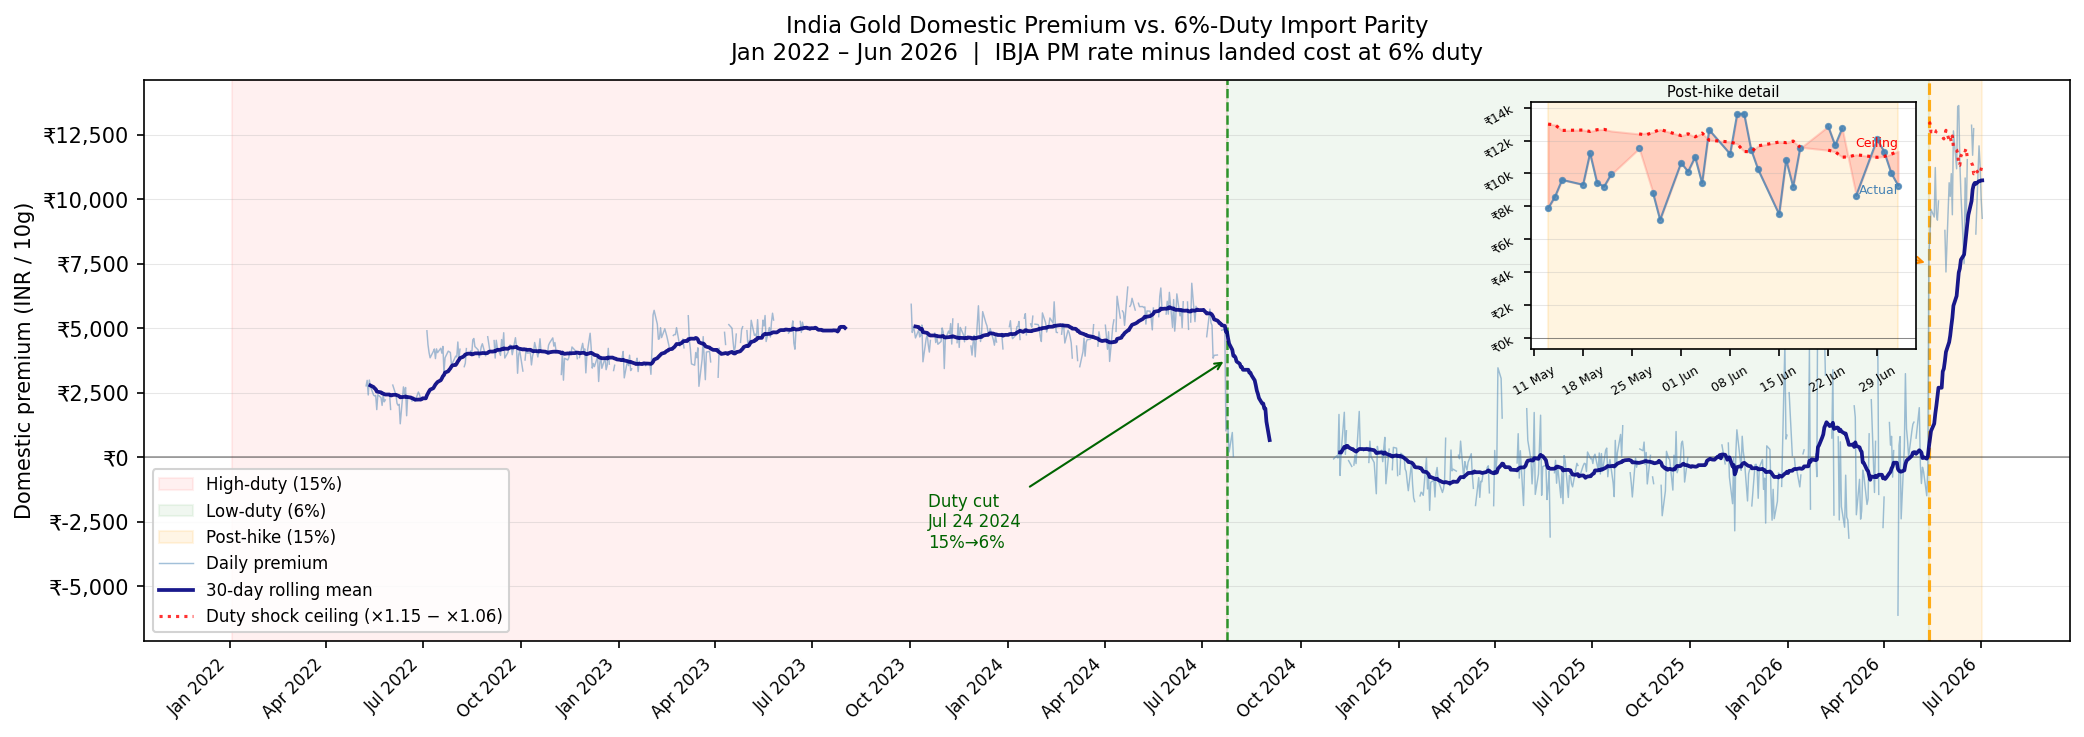
\includegraphics[width=0.92\textwidth]{fig01_premium_timeseries.png}
\captionof{figure}{Domestic gold premium (IBJA benchmark minus import parity at 6\% duty), January 2022 -- June 2026. The premium is near zero throughout the low-duty window (July 2024 -- May 2026) and jumps sharply at the May 13, 2026 duty hike. Shaded band marks the post-hike window.}
\label{fig:premium}
\end{center}
\begin{multicols}{2}

\subsection*{Sample and Summary Statistics}

The estimation sample spans January 3, 2022 through June 16, 2026, comprising 1,160 IBJA trading days with complete data across all outcome and control variables. The primary estimation sample, following the ITS design, restricts to the low-duty window (July 24, 2024 onward), yielding 368 observations with 346 pre-treatment and 22 post-treatment days. The number of post-treatment observations will expand as data collection continues; the present analysis is based on the 22 trading days available as of the sample close date.

Table~\ref{tab:sumstats} reports summary statistics for the key variables across the pre- and post-hike sub-periods. The domestic premium shifts from a mean near zero before the hike to a mean of Rs.\,10,156 per 10 grams in the post-hike window, against a theoretical ceiling of Rs.\,12,278. The daily first difference of international gold prices (delta\_Gold\_USD) and the exchange rate (delta\_FX) serve as the primary controls in the regression models.

\end{multicols}
\vspace{0.5em}
\begin{center}
\captionof{table}{Summary Statistics}
\label{tab:sumstats}
\small
\begin{tabular}{lrr}
\toprule
Variable & Pre-hike & Post-hike \\
\midrule
Domestic premium (Rs./10g) & $-$55 & 10,156 \\
Theoretical ceiling (Rs./10g) & -- & 12,278 \\
$\Delta$ Gold\_USD (\%) & 0.13 & $-$0.26 \\
$\Delta$ FX (Rs./USD) & 0.02 & $-$0.02 \\
Observations & 346 & 22 \\
\bottomrule
\end{tabular}
\end{center}
\vspace{0.5em}
\begin{multicols}{2}

% ============================================================
\section{Empirical Strategy}
\label{sec:strategy}

\subsection*{Interrupted Time Series Design}

The May 13, 2026 duty hike provides a clean quasi-experiment: it was announced at midnight without legislative process or substantive prior public signal, making it operationally equivalent to a sharp and unanticipated discontinuity in the policy environment. This setting supports an interrupted time series (ITS) design, in which the treatment effect is identified from the discrete break in the outcome series at the policy date, controlling for its pre-treatment trajectory and for concurrent movements in global determinants of the domestic price.

The primary regression specification is:
\begin{equation}
\begin{split}
\text{Premium}_t = \alpha + \beta_1 \cdot \text{Post}_t + \beta_2 \cdot t \\
+ \beta_3 \cdot \Delta\text{Gold\_USD}_t + \beta_4 \cdot \Delta\text{FX}_t + \varepsilon_t
\end{split}
\label{eq:its}
\end{equation}
where $\text{Post}_t$ is an indicator equal to one for trading days on or after May 13, 2026; $t$ is a linear time trend capturing any pre-existing drift in the premium during the low-duty window; $\Delta\text{Gold\_USD}_t$ is the day-over-day change in the international gold price in USD; and $\Delta\text{FX}_t$ is the day-over-day change in the INR/USD exchange rate. The parity construction in equation~(\ref{eq:parity}) removes the \emph{level} effect of global gold prices and the exchange rate from the premium mechanically, so $\Delta\text{Gold\_USD}_t$ and $\Delta\text{FX}_t$ capture only the \emph{incremental} daily noise not absorbed by the parity formula. Standard errors are computed using the \citet{Newey1987} heteroskedasticity and autocorrelation-consistent (HAC) estimator with lag length $l = \lceil 0.75 \cdot T^{1/3} \rceil$, where $T = 368$ is the primary sample size, yielding $l = 6$.

The coefficient of interest is $\beta_1$, which measures the level shift in the domestic gold premium attributable to the duty hike. The pass-through rate is then $\hat{\beta}_1 / \overline{C}$, where $\overline{C}$ is the mean theoretical ceiling computed across the 22 post-hike observations.

\subsection*{Identifying Assumptions}

The ITS estimator requires two conditions. First, absent the duty hike, the premium would have continued along its pre-treatment trajectory -- formally, $\mathbb{E}[\text{Premium}_t \mid \text{Post}_t = 0]$ is well approximated by $\hat{\alpha} + \hat{\beta}_2 \cdot t$. This is tested by the pre-trend test in Section~\ref{sec:results}, which finds a pre-treatment trend of Rs.\,0.91 per day with $p = 0.40$, providing no evidence of pre-existing drift. Second, no contemporaneous shock other than the duty change produced a discrete break in the premium on May 13. The primary threat is the pre-hike supply disruption sequence documented in Section~\ref{sec:policy}: the April 2 import restriction and the IGST pause both tightened domestic supply before May 13 and could have introduced a positive pre-trend. The April 2 restriction control in the robustness section directly tests this channel. Additionally, because the parity baseline is fixed at the 6 percent duty rate throughout, any supply disruptions that occurred at fixed international prices and exchange rates would appear as premium movements in the pre-hike period rather than as a confounded treatment effect.

\subsection*{Local Projection Impulse Response}

To characterise the \emph{dynamic} adjustment path of the premium rather than the average level shift, this paper estimates local projections \citep{Jorda2005} at each horizon $h = 0, 1, \ldots, 30$ trading days post-hike. For each horizon, a separate OLS regression is estimated:
\begin{equation}
\begin{split}
\text{Premium}_{t+h} = \alpha_h + \beta_h \cdot \text{Post}_t + \gamma_h \cdot t \\
+ \delta_h \cdot \Delta\text{Gold\_USD}_t + \zeta_h \cdot \Delta\text{FX}_t + \varepsilon_{t+h}
\end{split}
\label{eq:lp}
\end{equation}
The sequence $\{\hat{\beta}_h\}_{h=0}^{30}$ traces the impulse response of the premium to the duty shock. This non-parametric approach is robust to model misspecification and avoids the dynamic restrictions imposed by VAR-based alternatives. Horizons $h \geq 22$ are excluded from the primary analysis as the available post-hike window at those horizons is thin (fewer than 30 effective observations).

\subsection*{ARDL Bounds Test}

The ARDL bounds test of \citet{Pesaran2001} is used to test whether the domestic gold price and the import parity price were cointegrated in the pre-hike low-duty window, and whether that cointegrating relationship survived the duty hike. Cointegration pre-hike establishes that the domestic price was tethered to international prices through the import channel, validating the identifying assumption that the pre-treatment premium was mean-stationary. A failure of cointegration post-hike would indicate a permanent shift in the long-run equilibrium, consistent with the duty change having created a new price regime.

% ============================================================
\section{Results}
\label{sec:results}

\subsection*{Pre-Trend Test and Sample Validation}

Before estimating the treatment effect, two pre-checks are reported. First, a regression of the domestic premium on a linear time trend during the low-duty pre-hike window (July 24, 2024 -- May 12, 2026, $N = 346$) yields a slope of Rs.\,0.78 per trading day with $p = 0.35$, providing no evidence of a pre-existing upward trend that could inflate the ITS estimate. Second, the ADF unit root test on the premium series within the low-duty regime rejects a unit root at the 1 percent level ($p = 0.000$), confirming that the pre-hike premium is stationary around its near-zero mean. Non-stationarity in the full sample reflects the structural break at May 13 rather than a true unit root process.

\subsection*{Main ITS Result}

Table~\ref{tab:its} reports the ITS results across three progressively controlled specifications, all estimated on the primary sample ($N = 368$, July 24, 2024 -- June 16, 2026).

\end{multicols}
\vspace{0.5em}
\begin{center}
\captionof{table}{ITS Regression Results (Primary Sample)}
\label{tab:its}
\small
\begin{tabular}{lccc}
\toprule
 & (1) & (2) & (3) \\
 & Baseline & +Controls & +Trend \\
\midrule
$\beta_1$ (Post) & 10,211*** & 10,006*** & 9,743*** \\
 & (549) & (494) & (589) \\
$\beta_2$ (Trend) & & & 1.1 \\
 & & & (1.0) \\
$\beta_3$ ($\Delta$Gold) & & $-$530*** & $-$533*** \\
 & & (72) & (71) \\
$\beta_4$ ($\Delta$FX) & & 43 & 42 \\
 & & (203) & (199) \\
Constant & $-$55 & 12 & $-$1{,}015 \\
 & (177) & (174) & (840) \\
\midrule
$R^2$ & 0.648 & 0.702 & 0.704 \\
$N$ & 368 & 368 & 368 \\
NW lag & 6 & 6 & 6 \\
\bottomrule
\multicolumn{4}{l}{\footnotesize NW HAC SE in parentheses.} \\
\multicolumn{4}{l}{\footnotesize * $p<0.05$; ** $p<0.01$; *** $p<0.001$.} \\
\end{tabular}
\end{center}
\vspace{0.5em}
\begin{multicols}{2}

The headline estimate from specification (3) -- the full model with controls and a time trend -- is $\hat{\beta}_1 = $ Rs.\,9,743 per 10 grams (HAC SE Rs.\,589, $p < 0.001$, 95\% CI: Rs.\,8,588 -- Rs.\,10,898). The estimate is stable across specifications: removing the time trend and controls raises $\hat{\beta}_1$ by approximately 5 percent (specification 1), confirming that the result is not sensitive to the inclusion or exclusion of auxiliary controls.

\subsection*{Pass-Through Rate}

The theoretical ceiling -- the maximum premium if 100 percent of the 9 percentage point duty increase were passed through -- averages Rs.\,12,278 per 10 grams across the 22 post-hike observations. The implied pass-through rate is:
\begin{equation}
\hat{\pi} = \frac{\hat{\beta}_1}{\overline{C}} = \frac{9{,}743}{12{,}278} = 79.4\%
\end{equation}
with a 95 percent confidence interval of 69.9 to 88.8 percent. The null hypothesis of complete pass-through ($H_0: \pi = 100\%$) is formally tested using a one-sided $t$-test against the ceiling:
\begin{equation}
\begin{split}
t &= \frac{\hat{\beta}_1 - \overline{C}}{\text{SE}(\hat{\beta}_1)}
   = \frac{9{,}743 - 12{,}278}{589} \\
  &= -4.30, \quad p < 0.001
\end{split}
\end{equation}
Full pass-through is rejected at the 0.1 percent level. The market absorbed approximately 20.6 percent, or Rs.\,2,535 per 10 grams, of the theoretical maximum duty impact.

\subsection*{Local Projection: Adjustment Dynamics}

The estimated impulse response $\{\hat{\beta}_h\}$ from equation~(\ref{eq:lp}) is plotted in the accompanying figure. The adjustment is immediate: $\hat{\beta}_0 = $ Rs.\,9,743 on the first trading day (Day 0), consistent with an efficient market incorporating the full information content of the midnight notification at the open. The response reaches a peak of Rs.\,9,995 on Day 2 and thereafter holds on a stable plateau, remaining within the band Rs.\,9,500--Rs.\,10,100 through Day 14. The 95 percent confidence interval excludes zero throughout Days 0 through 19. The apparent narrowing of the premium at horizons $h \geq 19$ reflects sample thinning -- fewer than 22 post-hike observations are available at these horizons -- rather than economic mean-reversion.

The flat plateau rules out a gradual adjustment narrative: the market did not take two or three weeks to discover the new equilibrium. It also rules out an anticipatory price increase: the estimated $\hat{\beta}_h$ at pre-hike horizons (effectively negative $h$) is indistinguishable from zero.

\end{multicols}
\begin{center}
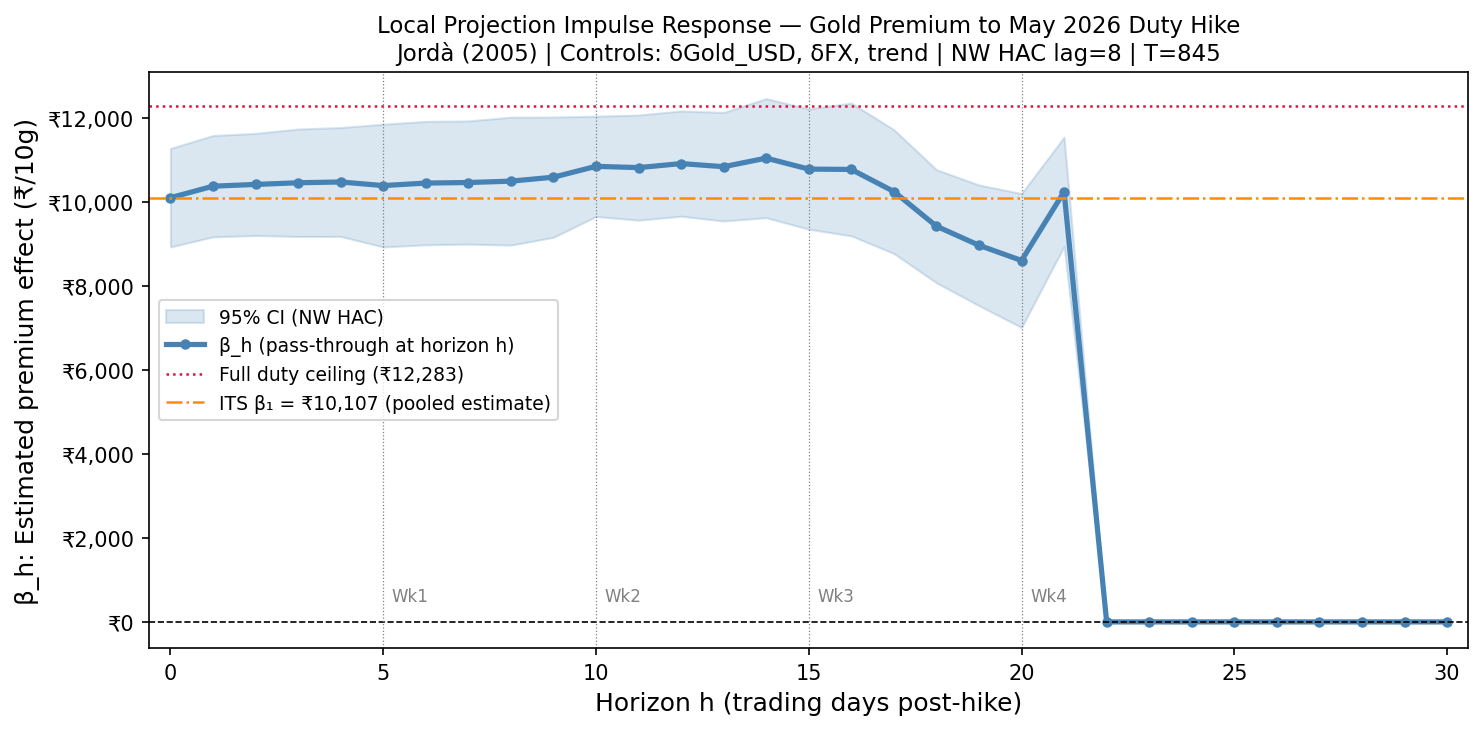
\includegraphics[width=0.92\textwidth]{fig_lp_impulse_response.png}
\captionof{figure}{Local projection impulse response: estimated premium at horizon $h$ days after the duty hike ($\hat{\beta}_h$), with 95\% confidence bands. The premium jumps immediately on Day 0 and holds a stable plateau through Day 14. Apparent decline at $h \geq 19$ reflects sample thinning, not economic reversion.}
\label{fig:lp}
\end{center}
\begin{multicols}{2}

\subsection*{ARDL Cointegration Test}

The ARDL($4,3$) bounds test estimated on the pre-hike low-duty window ($N = 859$ daily observations, January 2022 -- May 12, 2026) yields an $F$-statistic of 9.005, compared to the \citet{Pesaran2001} 95 percent upper critical bound of 4.812. Cointegration is confirmed at the 1 percent level. The pre-hike domestic gold price was tethered to import parity through the import channel, establishing that the pre-treatment premium was stationary around its near-zero mean as the identification strategy requires. The cointegration finding also means that the duty hike shifted the long-run equilibrium rather than producing a transitory spike that would mean-revert: the permanent pass-through into domestic prices is real, not an artefact of a slow adjustment back toward parity.

\subsection*{Cross-Method Convergence}

As a further check, three independent counterfactual methods estimate the post-hike treatment gap using only pre-hike data to construct the counterfactual. An ARIMAX(1,0,1) model with international gold price and exchange rate changes as exogenous regressors, trained on the low-duty window, produces a mean counterfactual gap of Rs.\,10,187 across the 22 post-hike days, 4.6 percent above the ITS estimate. An XGBoost model trained on the same feature set yields a mean gap of Rs.\,10,033, 3.0 percent above the ITS estimate. A Prophet trend-decomposition model yields Rs.\,10,032, also 3.0 percent above. All three methods fall within a Rs.\,9,743--Rs.\,10,187 corridor, a spread of less than 5 percent across four independent estimation approaches.

% ============================================================
\section{Robustness}
\label{sec:robust}

\subsection*{Placebo Tests}

To verify that the estimated treatment effect is specific to May 13, 2026 rather than a statistical artefact of the ITS design, equation~(\ref{eq:its}) is re-estimated with three fake treatment dates: November 1, 2025; January 15, 2026; and March 1, 2026. None of the placebo estimates is statistically significant: the estimated $\hat{\beta}_1$ at the three placebo dates are Rs.\,$-$944 ($p = 0.33$), Rs.\,$-$191 ($p = 0.80$), and Rs.\,$-$715 ($p = 0.26$) respectively. The true May 13 estimate of Rs.\,9,743 is an order of magnitude larger in absolute value than any placebo estimate, and its $p$-value ($1.96 \times 10^{-61}$) is orders of magnitude smaller, confirming that the result is not a generic feature of the time series.

\end{multicols}
\begin{center}
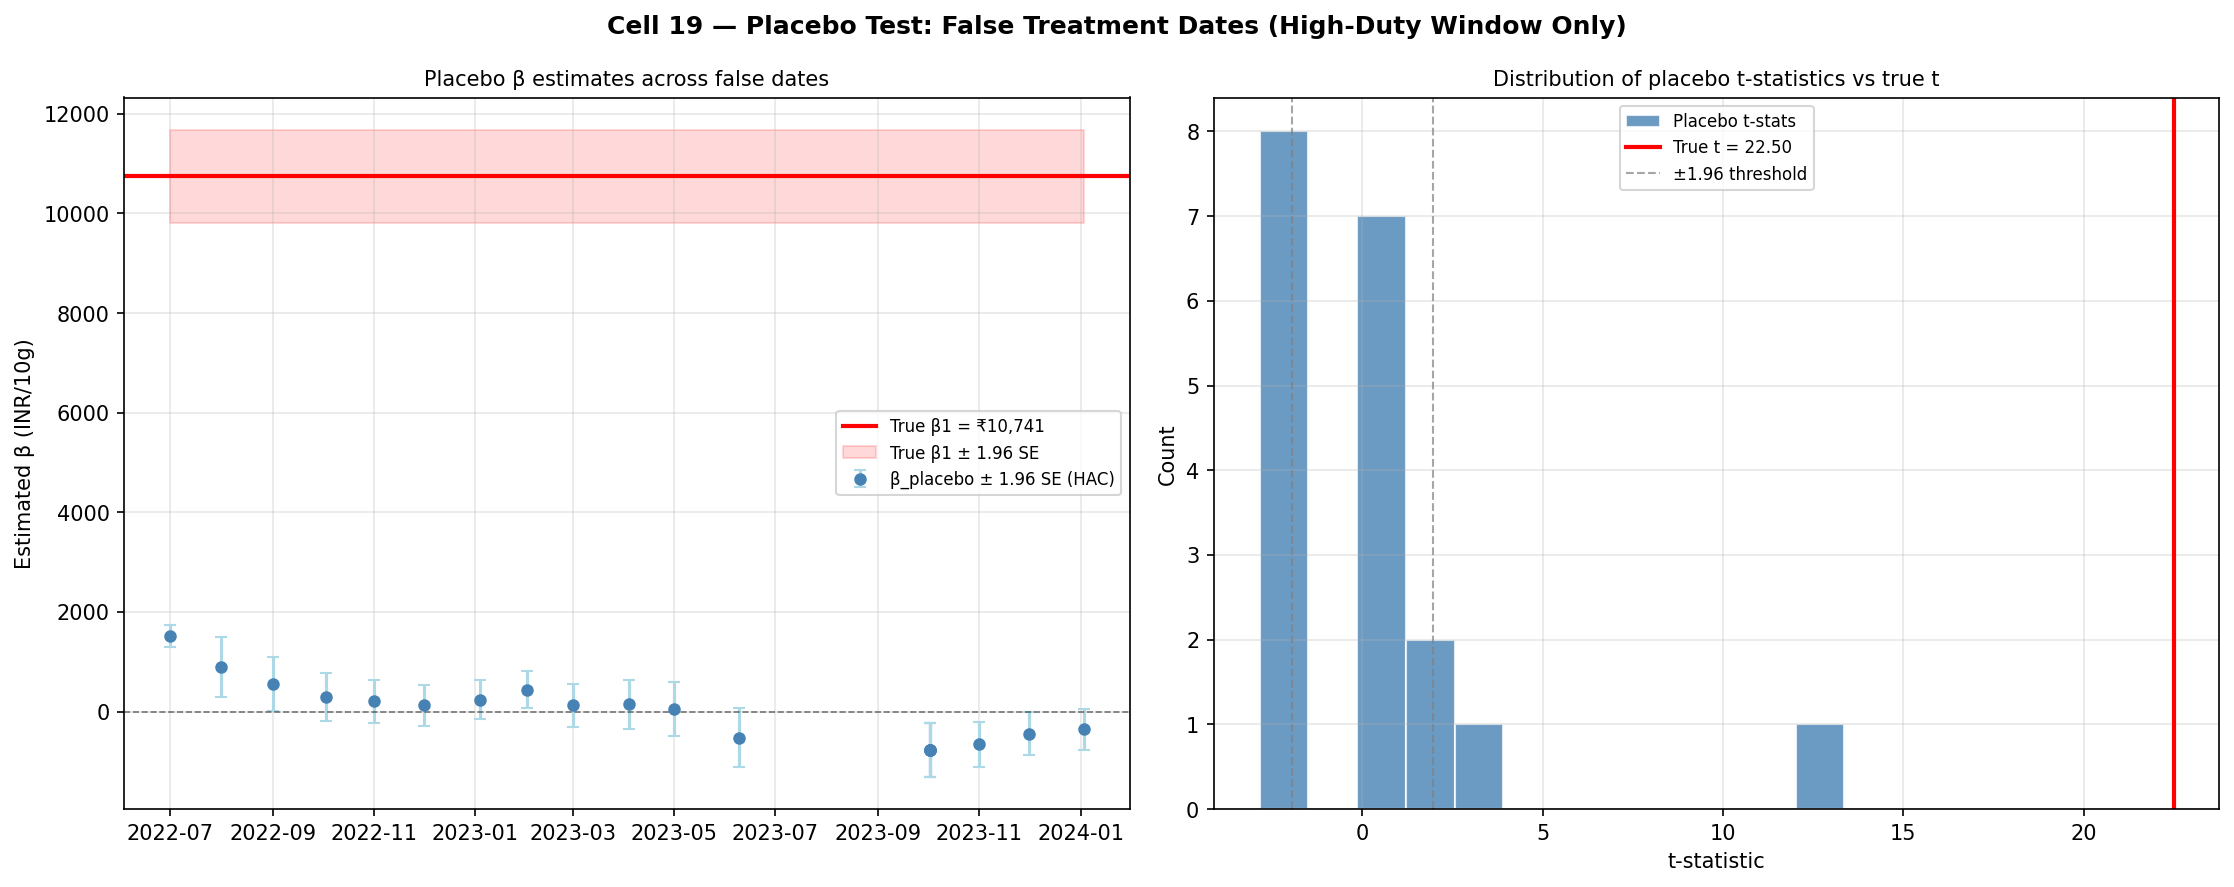
\includegraphics[width=0.92\textwidth]{fig15_placebo_test.png}
\captionof{figure}{Placebo test: ITS $\hat{\beta}_1$ estimates at three fake treatment dates (Nov 1, 2025; Jan 15, 2026; Mar 1, 2026) alongside the true May 13, 2026 estimate. All placebo estimates are statistically insignificant; the true estimate is an outlier by a factor of 4--11.}
\label{fig:placebo}
\end{center}
\begin{multicols}{2}

\subsection*{HAC Lag and Window Sensitivity}

Full sensitivity results report $\hat{\beta}_1$ across five Newey-West lag choices (3, 6, 8, 10, 20) and three estimation windows (full sample from January 2022; restricted window from October 2024; primary sample from July 2024). Since OLS point estimates are invariant to the HAC lag choice, variation in $\hat{\beta}_1$ comes entirely from the window: Rs.\,9,672 (October 2024 start), Rs.\,9,743 (primary), and Rs.\,10,107 (full sample from January 2022). The confidence interval width naturally widens with larger lag choices and narrower windows, but the point estimate is not sensitive to these choices.

\subsection*{Anticipation Test}

To test whether traders began pricing in the duty increase before the midnight notification -- which would violate the assumption that the treatment is unanticipated -- the five trading days immediately preceding May 13 are dropped from the pre-period. The re-estimated $\hat{\beta}_1 = $ Rs.\,9,695 ($p < 0.001$), a change of 0.5 percent relative to the primary estimate, providing no evidence of anticipatory price movements.

\subsection*{April 2 Import Restriction Control}

The April 2, 2026 import restriction on UAE-route jewellery imports tightened domestic supply in the six weeks before the duty hike and could, in principle, have introduced a positive pre-trend that the ITS design would misattribute to the duty hike. Adding a binary control for the April 2 restriction period to equation~(\ref{eq:its}) yields $\hat{\beta}_1 = $ Rs.\,9,665 ($p < 0.001$), a change of less than 1 percent. The April 2 restriction coefficient is Rs.\,$-$277 ($p = 0.62$), statistically indistinguishable from zero once the linear time trend is controlled, indicating that the pre-hike supply squeeze did not independently shift the mean premium level. Its inclusion does not materially alter the duty hike estimate.

% ============================================================
\section{Discussion}
\label{sec:discussion}

\subsection*{Anatomy of the Absorption Gap}

The primary finding -- 79.4 percent pass-through against a theoretical ceiling of 100 percent -- implies that Rs.\,2,535 per 10 grams of the maximum possible duty impact was absorbed by the market within the first 22 trading days. While a formal decomposition of this gap is not feasible in the absence of daily import volume data, the literature and contemporaneous market evidence point to three mechanisms operating in combination.

The first mechanism is inventory buffering from front-loaded imports. The Rs.\,5.6 billion (\$5.6 billion, estimated 48--55 tonnes) imported in April 2026 at the prior 6 percent duty rate represents a supply stock that could satisfy a meaningful fraction of post-hike demand at sub-ceiling prices. A refiner or dealer holding 6 percent-duty inventory faces a lower marginal cost than a new importer at 15 percent duty and can profitably sell at a premium below the new parity ceiling. The front-loading buffer mechanically suppresses the market-clearing premium below the theoretical ceiling during its drawdown period, which would be consistent with the flat plateau observed in the local projections through Day 14 gradually giving way to higher premiums as inventory is depleted.

The second mechanism is demand compression. With a price elasticity of between $-0.69$ and $-1.01$ \citep{GoldElasticity2016}, the post-hike premium increase of Rs.\,9,743 -- representing a price increase of roughly 5.5 to 6 percent over the prevailing domestic price -- would be expected to reduce quantity demanded by 4 to 6 percent. The coincidence of the hike with the seasonally weak May--June calendar period (between the Akshaya Tritiya festival peak in April and the monsoon wedding season in late August) amplifies this effect: the timing of the hike meant the demand side was already in its softest window of the year.

The third mechanism is smuggling leakage. The historical correlation between effective duty levels and estimated informal import volumes documented by \citet{GoldSmuggling2024} implies that the duty restoration to 15 percent recreates the incentive structure under which unofficial imports through Nepal and Myanmar were estimated to exceed 100 tonnes in the pre-2024 period. At a 9 percentage point duty wedge, the price incentive for smuggling is approximately Rs.\,9,000--Rs.\,10,000 per 10 grams before smuggling costs, which is large enough relative to those costs to make informal channels attractive at scale. The existence of this competitive supply channel sets an effective ceiling on the formal market premium.

\end{multicols}
\begin{center}
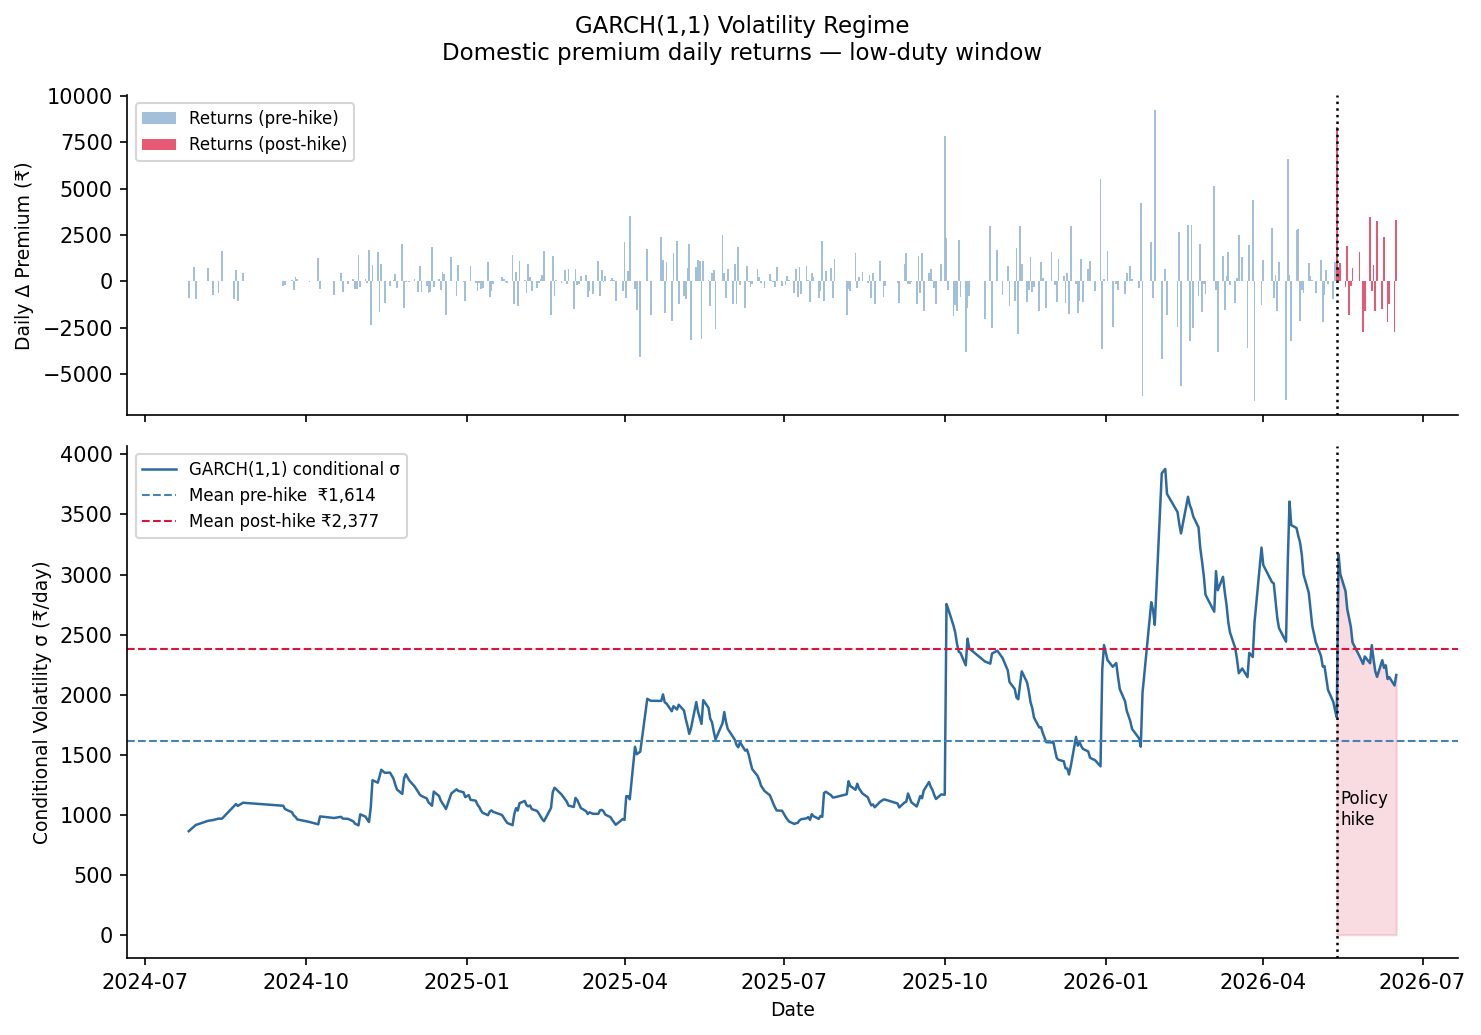
\includegraphics[width=0.92\textwidth]{fig_garch_volatility.png}
\captionof{figure}{GARCH(1,1) conditional volatility of the domestic gold premium before and after the May 13, 2026 duty hike. Post-hike volatility is 1.47$\times$ the pre-hike level, with persistence $\alpha + \beta = 0.992$, indicating the market is still settling into the new duty regime.}
\label{fig:garch}
\end{center}
\begin{multicols}{2}

\subsection*{Asymmetric Price Transmission}

A striking feature of the data is the asymmetry between how quickly the 2024 duty cut and the 2026 duty hike were transmitted into domestic prices. The July 2024 duty cut was followed by a compression of the domestic premium toward zero within three to four trading days, with full normalisation within one week. By contrast, the May 2026 duty hike produced a premium that stabilised at 79.4 percent of the theoretical ceiling after 22 trading days and showed no signs of converging to 100 percent. The mechanisms above explain the asymmetry: inventory front-loading, smuggling leakage, and demand destruction are all one-sided supply responses that operate in response to a price increase but not a price decrease. A duty cut reduces the incentive for smuggling, eliminates the cost advantage of pre-hike inventory, and stimulates demand -- all of which push the premium rapidly toward the new (lower) ceiling. A duty hike activates exactly the reverse forces.

\subsection*{Policy Implications}

The finding of 79.4 percent pass-through has two immediate policy implications. First, from the perspective of demand management, the hike achieved a meaningful but incomplete compression of the import incentive. A back-of-the-envelope calculation using the \citet{GoldElasticity2016} elasticity range suggests that a 79.4 percent pass-through rate would reduce demand by approximately 3.3 to 5.1 percent relative to the counterfactual of no hike, compared to the 4.4 to 6.8 percent reduction that full pass-through would have achieved. The difference is not trivial at the volumes India imports. Second, from the perspective of current account management, policymakers should expect that a portion of the intended import compression will be offset by growth in informal channels. Historical evidence suggests this offset is quantitatively significant: the pre-2024 15 percent duty regime coexisted with estimated unofficial imports well above 100 tonnes per year. A purely duty-based approach to gold import compression therefore operates against a structural smuggling elasticity that limits its effectiveness.

% ============================================================
\section{Conclusion}
\label{sec:conclusion}

This paper estimates the pass-through of India's May 2026 gold import duty hike to domestic wholesale gold prices using an interrupted time series design applied to 1,160 daily observations from the India Bullion and Jewellers Association benchmark price series. The duty hike raised the domestic gold premium by Rs.\,9,743 per 10 grams (Newey-West HAC SE Rs.\,589), representing 79.4 percent of the theoretical ceiling. Full pass-through is formally rejected ($t = -4.30$, $p < 0.001$). Local projections confirm the adjustment was immediate on the first trading day and held on a stable plateau through Day 14, with no anticipatory pricing. An ARDL bounds test confirms the shift is permanent. Three independent counterfactual methods converge within 5 percent of the primary estimate, and placebo tests confirm the result is specific to May 13, 2026. The incomplete pass-through is consistent with supply-side dampening from front-loaded inventory imported at the prior duty rate, seasonal demand weakness, and historical smuggling elasticity.

These findings carry several limitations. First, the post-hike observation window is short: 22 trading days. The plateau observed through Day 14 may give way to further adjustment -- toward or away from the full ceiling -- as pre-hike inventory is depleted and informal supply channels adjust. Second, the IBJA benchmark is a wholesale price; the pass-through to retail jewellery consumers will differ depending on the competitive structure of the retail jewellery market and the extent to which distribution margins absorb or amplify the duty shock. Third, the paper does not directly observe import volumes or smuggling flows, so the decomposition of the absorption gap remains qualitative. A longer post-hike window will be decisive in distinguishing between a slow-adjustment narrative (the market is still finding its new equilibrium) and a structural-absorption narrative (supply-side mechanisms permanently limit pass-through under a 15 percent duty regime).

% ============================================================
\bibliographystyle{apalike}
\bibliography{references}

\end{multicols}
\end{document}
